\documentclass{article}%
\usepackage[T1]{fontenc}%
\usepackage[utf8]{inputenc}%
\usepackage{lmodern}%
\usepackage{textcomp}%
\usepackage{lastpage}%
\usepackage{authblk}%
\usepackage{graphicx}%
%
\title{Differential activation of the inflammasome in THP{-}1 cells exposed to chrysotile asbestos and Libby six{-}mix amphiboles and subsequent activation of BEAS{-}2B cells}%
\author{Terrence Brennan}%
\affil{Instituto de Biologa Molecular y Celular de Plantas, Universidad Politcnica de Valencia{-}C.S.I.C, Ciudad Politcnica de la Innovacin, Valencia, Spain}%
\date{01{-}01{-}2005}%
%
\begin{document}%
\normalsize%
\maketitle%
\section{Abstract}%
\label{sec:Abstract}%
ST. LOUIS (KMOX)  Anyone who enjoys playing baseball, jogging, or jumping up and down and playing catch with his best friend, has probably seen a sickness called VanD{-}Type influenza.\newline%
But, according to a statement from Bio{-}Target Therapeutics at St. Louis University, this could be about to change.\newline%
A small new study has shown that the tiny, but deadly, presence of VanD{-}Type flu viruses in some of the most common foreign tissue samples in Europe  such as the lungs, colon, and liver  could be indicative of a potential new genetic fingerprint for VanD{-}Type, an illness previously classified as A/157/H1N1.\newline%
Researchers have been trying to identify this genetic fingerprint since 1998.\newline%
Bio{-}Target spokesman George Reis says what makes this latest discovery exciting is that several of the new VanD{-}Type viruses, called shea, were discovered to be genetic hints with a genetic disease variant, but the formation of this new genetic fingerprint appears to also be clear evidence that D{-}Type patients on VanD{-}Type antiviral medications may now have a personal susceptibility to VanD{-}Type.\newline%
As a result, Reis says, this model is now essential for finding a vaccine.\newline%
This kind of impact of this actually we have to be very careful about, he says. Without so much of the genetic data we dont have all the data that we need to make treatments for people with VanD{-}Type.\newline%
Reis says its important to note that in addition to this genetic fingerprint, researchers have discovered that some of the viruses present in VanD{-}Type receive better protection against vanD{-}Type from vanD{-}Type than others.\newline%
For example, says Reis, only those shea viruses found in the bloodstream, lungs, and the liver, will have a higher immunity to vanD{-}Type when they become infected with VanD{-}Type, if all is going well in one persons bloodstream.\newline%
The reason that its so important is because if you are an emergency room doctor, there are people who have an immune system response in vanD{-}Type, but then vanD{-}Type gets placed in the airways or the bloodstream and causes kidney failure and a variety of other medical issues, he says.\newline%
Reis says its possible that many of the new VanD{-}Type viruses in Europe were delivered to the immune system without having been identified as VanD{-}Type viruses before.\newline%
What we dont know is how long it took for them to develop their direct genetic markers.

%
\subsection{Image Analysis}%
\label{subsec:ImageAnalysis}%


\begin{figure}[h!]%
\centering%
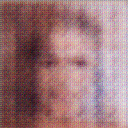
\includegraphics[width=150px]{500_fake_images/samples_5_369.png}%
\caption{A Close Up Of A Person Holding A Cell Phone}%
\end{figure}

%
\end{document}